\documentclass[Nomencl]{SelimArticle}
%!TEX root = main.tex

%%%%%%%%%%%%%%%%%%%%%%%%%%%%%%%
% Additional Packages/Options %
%%%%%%%%%%%%%%%%%%%%%%%%%%%%%%%
% \setlist{nosep}
\hypersetup{hidelinks}

%%%%%%%%%%%%%%%%%
% Title Options %
%%%%%%%%%%%%%%%%%
\usepackage{mypage}
\school{UC Santa Cruz}
\course{CE241}
\coursenum{Course Code}
%Add \\[0.3cm] for new line.
\title{Closed Loop Position Control for Characterizing Noise in Motion Capture Systems}
\student{Ryan \textsc{Rodriguez}}
\studentnum{1336732}
\date{\today}

%%%%%%%%%%%%%%%%%%%%%%%%%
% Additional Formatting %
%%%%%%%%%%%%%%%%%%%%%%%%%
%Horizontal line below section.
\sectionfont{\sectionrule{0pt}{0pt}{-5pt}{0.8pt}}
%Section numbering depth. Value of 2 means numbering ends with subsections.
\setcounter{secnumdepth}{3}
%Table of contents section depth. Same as above.
\setcounter{tocdepth}{2}
\numberwithin{equation}{section}
\numberwithin{figure}{section}
\newcommand{\ra}[1]{\renewcommand{\arraystretch}{#1}}

\usepackage{graphicx}
\usepackage{caption}
\usepackage{subcaption}
\graphicspath{ {./figs/} }
\DeclareGraphicsExtensions{.pdf,.png,.jpg}

\begin{document}
\mytitlepage
\tableofcontents
\newpage
\printnomenclature % Use makeidx.bat followed by two pdflatex reruns.
\newpage
% Begin writing here.

\section{Motivation}
Over the past several years, the application of infrared motion captures systems to the design and validation of control laws for a wide variety of problems. Although the server applications that accompany these systems include faculties for determining mean error based on a simple calibration step, it may often be the case that control engineers may want to verify their 'ground truth' based on more empirical evidence.

The focus of my project was on the design of  a closed loop positioning platform to be used in characterization of motion capture system noise. This was done using aluminum extrusion coupled to stepper belt-drives, with the addition of closed loop control in the form of a 'flying-fader' a type of linear motorized potentiometer commonly used in audio control panel applications. 

The structure of the report is as follows: first, we begin with a quick overview of the simple model I've used to design the controller for my system. Next, I'll outline how I modeled the system in Matlab, and ultimately how I implemented the system using a microcontroller and some off the shelf parts. 


\section{Analysis}
Naturally, the design of this controller began with some mathematical analysis to specify the physical system to be controlled. In the case of the flying fader, the physical mechanism consists of a DC motor coupled to a belt with a pulley. The belt, stretched taught by pulley's on either end, one passive, one active, serves as an energy transfer mechanism to a small tab attached to the belt for positioning some object, typically a sliding knob. My work was guided by work in\cite{beltModeling}, where thorough analysis of friction and controllers for the belt drive system were conducted.

The dynamics for the motor are given as follows:
\begin{equation}
G(s) = \frac{\dot{\Theta(s)}}{V(s)} = \frac{K}{(Js + b)(Ls+R)+K^2}~~ [\frac{rad/s}{V}]
\end{equation}

These follow naturally from Kirchoff and Newton:

\begin{equation*}
J\ddot{\theta} + b\dot{\theta} = Ki
L\frac{di}{dt} + Ri = V - K\dot{\theta}
\end{equation*}


The dynamics of the belt/pulley system are given as follows:
\begin{equation}
K_i=\frac{F_l}{\epsilon(l_i-x)}
\end{equation}
Where $F_i$ is the applied longitudinal force, $\epsilon$ is the strain, and $(l_i-x)$ is an added stretch term corresponding to the changing cart position.
The system transfer function is given by the simplified linear model:

\begin{align*}
J_M\ddot{\phi} &= \tau - RK_ew \\
M_c\ddot{x}&+k_v\dot{x}=K_ew \\
w&=R\phi - x
\end{align*}

Where $w$ is the belt stretch, $K_e$ is the elasticity of the belt, and $L=\frac{R}{G}$ is the transmission constant of the belt. From these equations, transfer functions relating torque to position of angular position of the motor may be obtained.

Given the model above, I implemented  the following system in Simulink:

\begin{align*}
J_M\ddot{\phi} &= \tau - RK_ew \\
M_c\ddot{x}&+k_v\dot{x}=K_ew \\
w&=R\phi - x
\end{align*}


\begin{figure}[!ht]
    \centering
    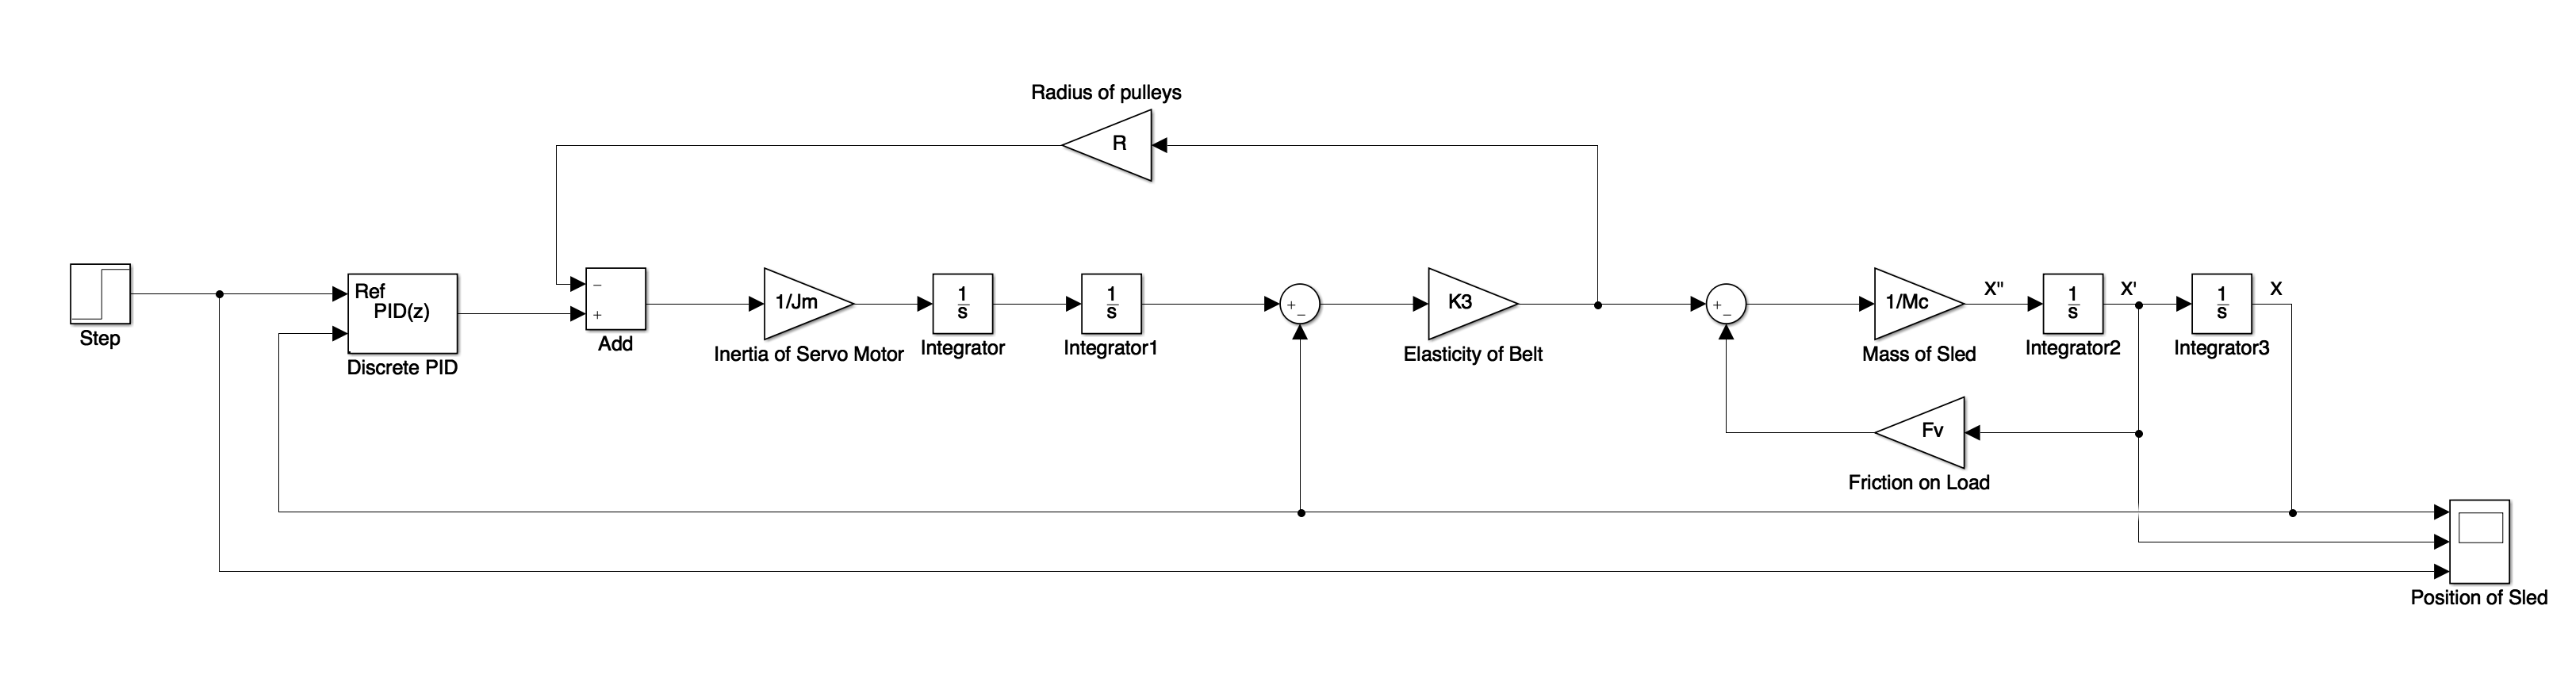
\includegraphics[width=\textwidth, height=2.75in]{simulink}
    \caption{Simulink model of the linearized belt drive system}
\end{figure}

Using the parameter tuning capabilities of Matlab, I modified the gains of the discrete PI controller to obtain a desired response with overshoot less than 20\%
and a rise time of less than 10ms.

\begin{figure}[!ht]
    \centering
    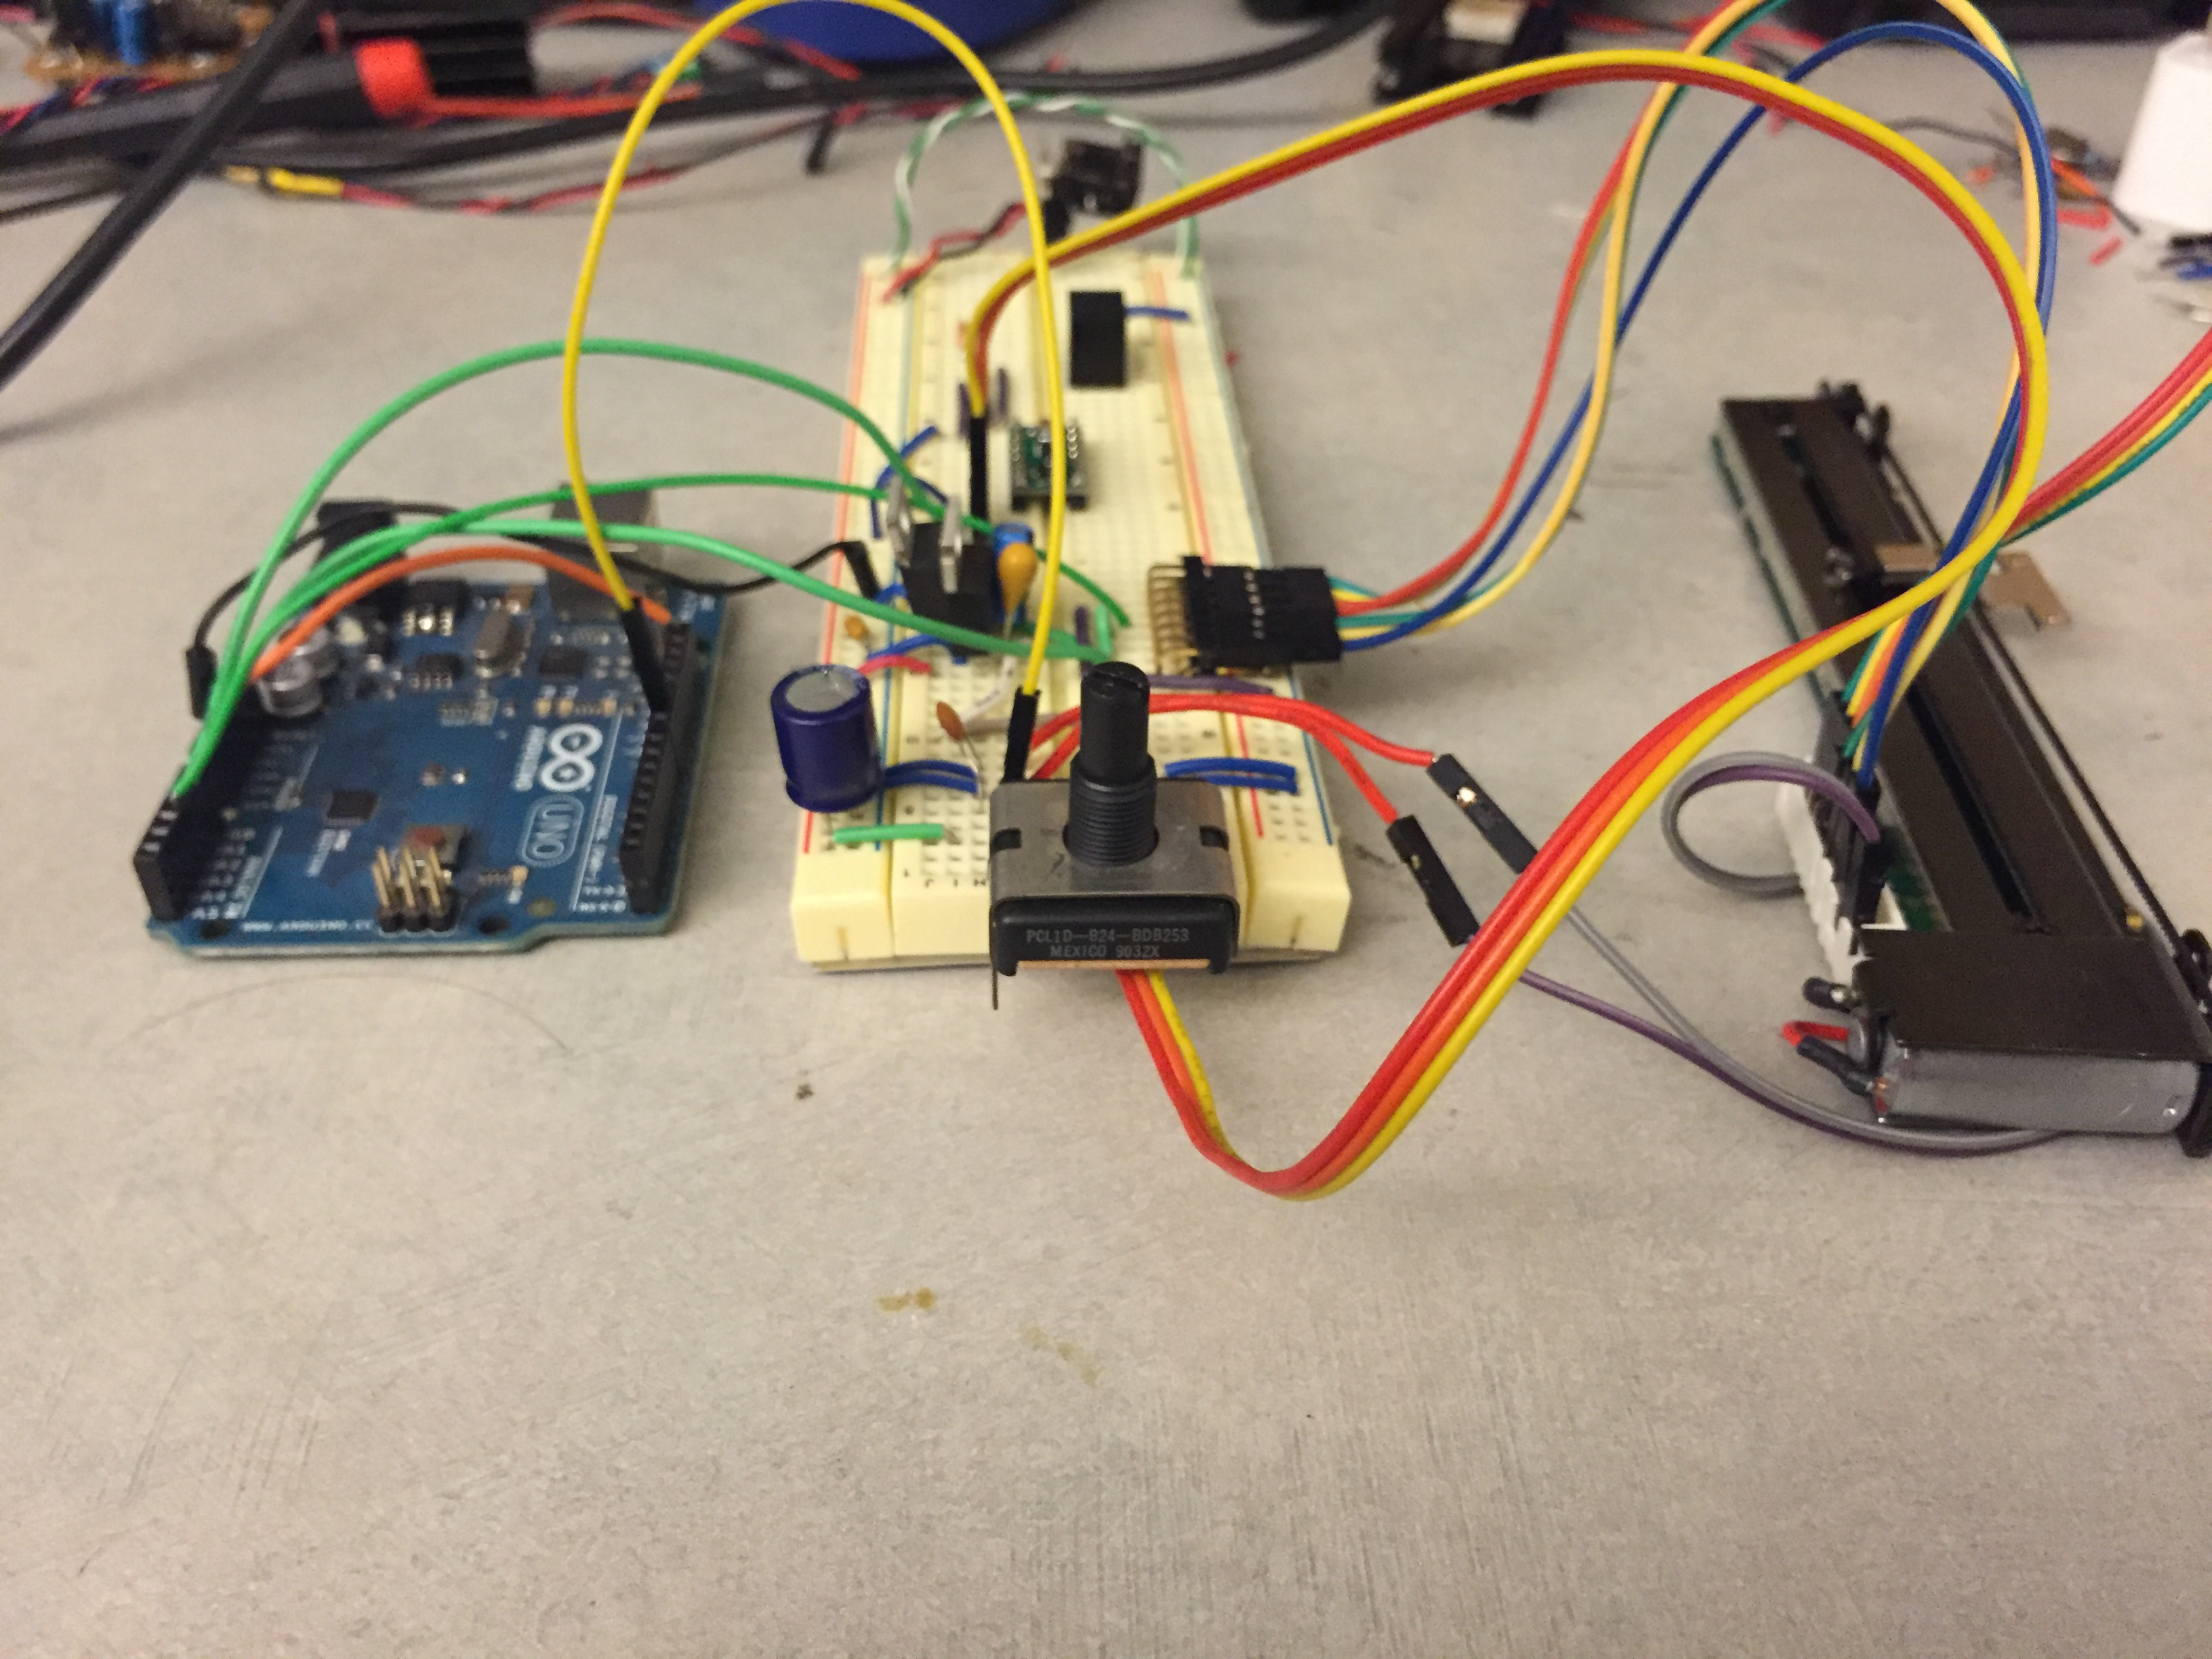
\includegraphics[width=\textwidth, height=3.5in]{exp1}
    \caption{The experimental setup: pictured is the discrete time PID implementation on an Atmel chip, with driver circuitry in the center, and the motorized pot on the right}
    \label{fig:exp1}
    
\end{figure}

\begin{figure}[!ht]
    \centering
    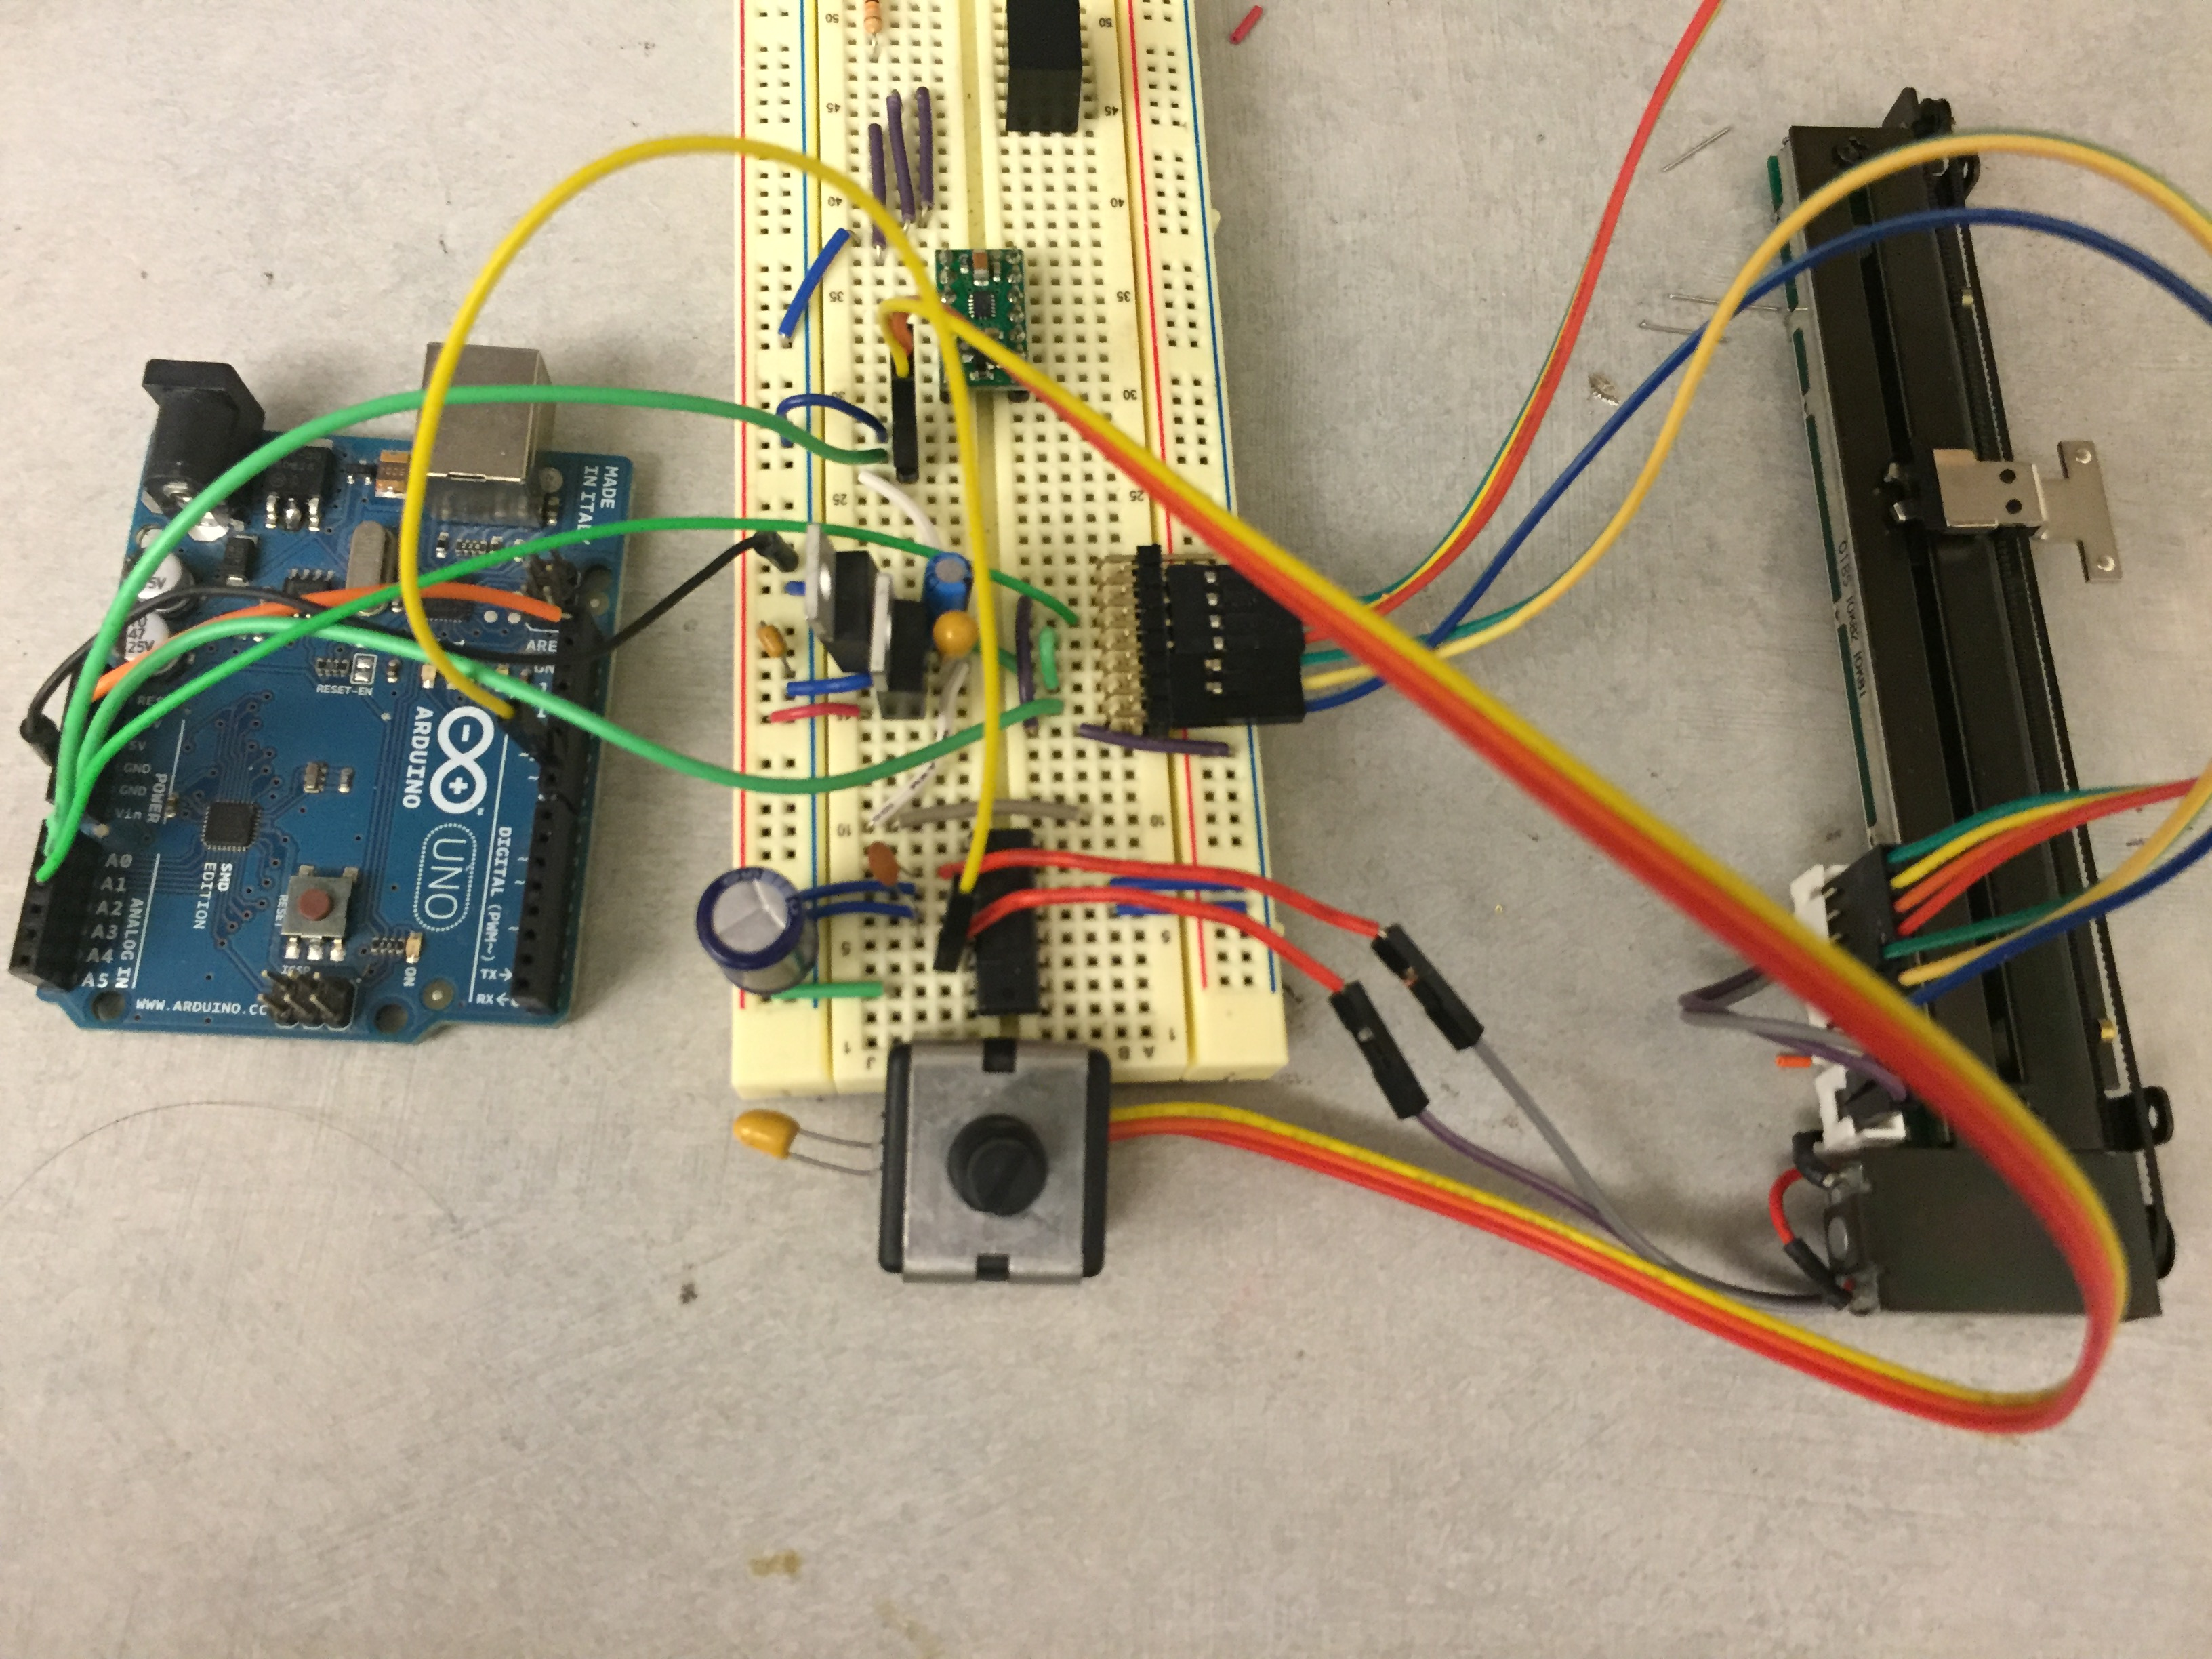
\includegraphics[width=\textwidth, height=3.5in]{exp2}
    \caption{The experimental setup: pictured is the discrete time PID implementation on an Atmel chip, with driver circuitry in the center, and the motorized pot on the right}
    \label{fig:exp2}
\end{figure}

To test this design on real hardware, I used the following experimental setup. Using an Atmel microcontroller, I implememented a simple discrete PID in C.
Using an off the shelf half-bridge driver (SN75044) and a motorized potentiometer, I constructed what is shown in Fig. \ref{fig:exp1} and Fig. \ref{fig:exp2}

From the model, the reponse obtained is shown in Fig.\ref{fig:response}
\begin{figure}[!ht]
    \centering
    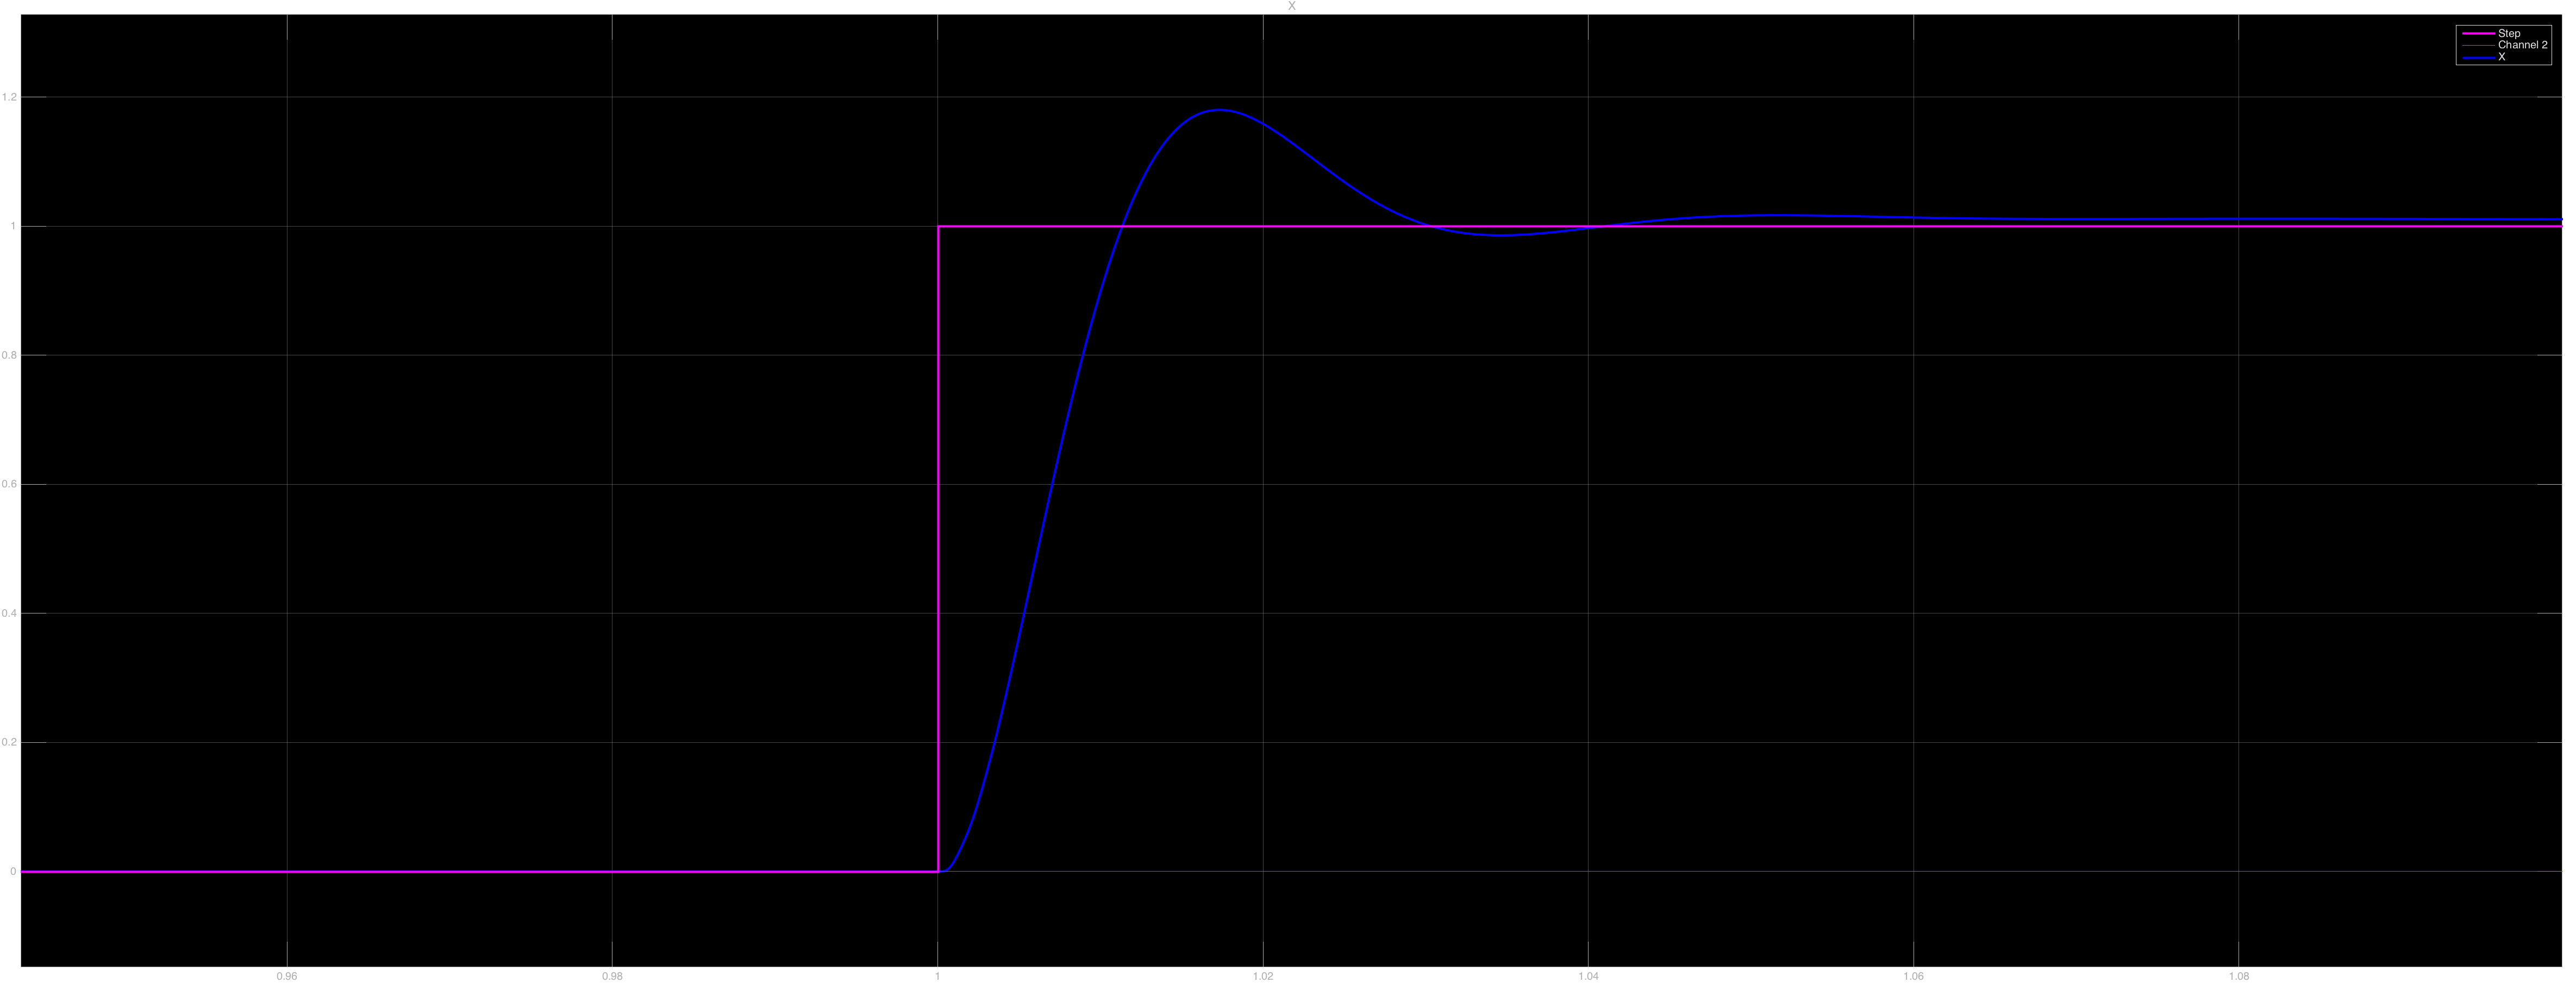
\includegraphics[width=\textwidth, height=2.75in]{response2}
    \caption{The response obtained from the model: step reference input is shown in magenta, the system output (position) is shown in blue}
    \label{fig:response}
\end{figure}

\section{Conclusion}
It has been shown that I performed an analysis of the system that took into consideration the dominant effects of the plant, namely the DC motor, inertial effects, and the elasticity of the belt. From these analyses, I implemented a Matlab Simulink model to tune a controller. Finally, I implemented the discrete controller on a microcontroller.



\bibliographystyle{IEEEtran}
\bibliography{main}
\end{document}